% start with a minimal latex template
\documentclass{article}
\usepackage{amsmath}
\usepackage{amssymb}
\usepackage{graphicx}
\usepackage{subfig}
% end of template

\begin{document}
\title{Whitebox Attack Using Neuron Outputs on Tabular Data}

\section{Threat Model}
\begin{itemize}
\item The attacker has access to a dataset $D=\{x_i,y_i\}_{i=1}^n$ with sensitive information $x_i^1,\ldots,x_i^m$ known.
\item The adversary has Whitebox access to the target model $f$ which means that the adversary knows the architecture of the model and the weights of the model. 
\end{itemize}

\section{Attack Strategy}
\begin{itemize}
    \item The adversary queries $f$ with $x_1, \ldots, x_n$ with the sensitive attribute set to the positive value and obtains the output of each hidden neuron $h_1, \ldots, h_k$ where $k$ is the number of hidden neurons. The query produces a matrix $M_1$ of size $n \times k$.
    \item The adversary queries $f$ again with the $n$ samples but this time using the negative value for the sensitive attribute. The query produces a matrix $M_2$ of size $n \times k$. $M_1$ and $M_2$ are concatenated to form a matrix $M$ of size $n \times 2k$.
    \item An attack model is trained with $M$ as the input features and $x^1$ as the target.
    \item During inference, the adversary queries $f$ with the partial record $x^2, \ldots, x^m$ twice once $x^1$ is set to the positive value and once it is set to the negative value. The output of the hidden neurons is concatenated to form a vector $v$ of size $2k$. Then the attack model is queried with $v$ to obtain the prediction of $x^1$.
\end{itemize}

\section{Comparison with Baseline Correlation Attack}
% include figure from plots/wb_comparison_w_baseline.png
\begin{figure}[h]
    \centering
    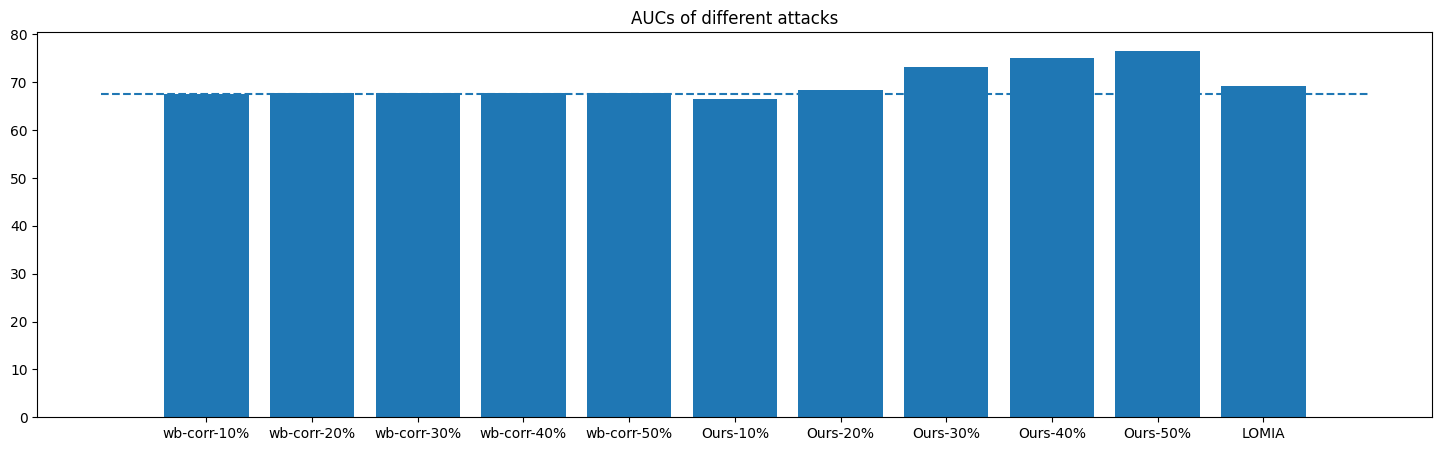
\includegraphics[width=0.8\textwidth]{plots/wb_comparison_w_baseline.png}
    \caption{Comparison of the proposed attack with the baseline correlation attack.}
    \label{fig:wb_comparison_w_baseline}
\end{figure}

Figure \ref{fig:wb_comparison_w_baseline} shows the comparison of the proposed attack with the baseline correlation attack.
The first $5$ bars from the left represents the AUC of correlation based baseline attack where the adversary has access to $10\%$, $20\%$, $30\%$, $40\%$, and $50\%$ of the training data respectively.
The performance is similar in all 5 scenarios.
This potentially indicates that the top-$10$ correlated neurons remain the same with different size of data available to the adversary.

The next $5$ bars from the left represents the AUC of the proposed attack where the adversary has access to $10\%$, $20\%$, $30\%$, $40\%$, and $50\%$ of the training data.
The performance of the proposed attack increases as the size of the data increases.
Only when the adversary has access to $10\%$ of the training data, the performance of the proposed attack is poor compared to the baseline attack.
But with increased amount of data available to the adversary, the performance of the proposed attack is significantly better than the baseline attack.

The final bar represents the case where our proposed attack is performed with LOMIA case 1 examples for which the adversary's prediction was correct.
This indicates that if the adversary has access to partial data and some way of finding which predictions are correct upon launching LOMIA, then that could be used to generate full records to be used in the proposed attack.


\section{Disparate Vulnerability Results}
% include figure from plots/disparate_vulnerability_1.png, plots/disparate_vulnerability_2.png, plots/disparate_vulnerability_3.png
\begin{figure}[h]
    \centering
    \subfloat[Disparate vulnerability of Sex]{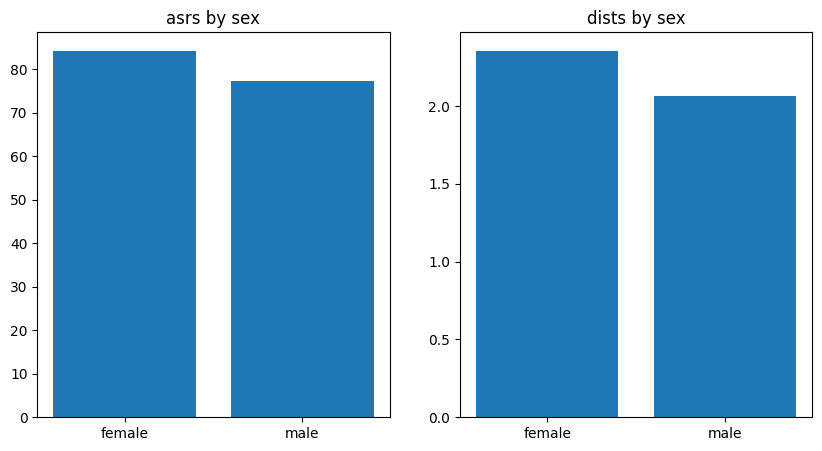
\includegraphics[width=0.33\textwidth]{plots/disparate_vulnerability_1.png}\label{fig:disparate_vulnerability_1}}
    \hfill
    \subfloat[Disparate vulnerability of Race]{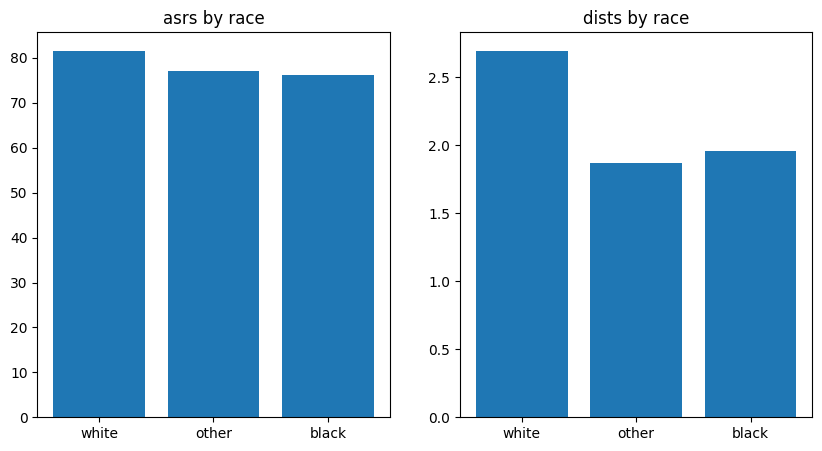
\includegraphics[width=0.33\textwidth]{plots/disparate_vulnerability_2.png}\label{fig:disparate_vulnerability_2}}
    \hfill
    \subfloat[Disparate vulnerability of Religion]{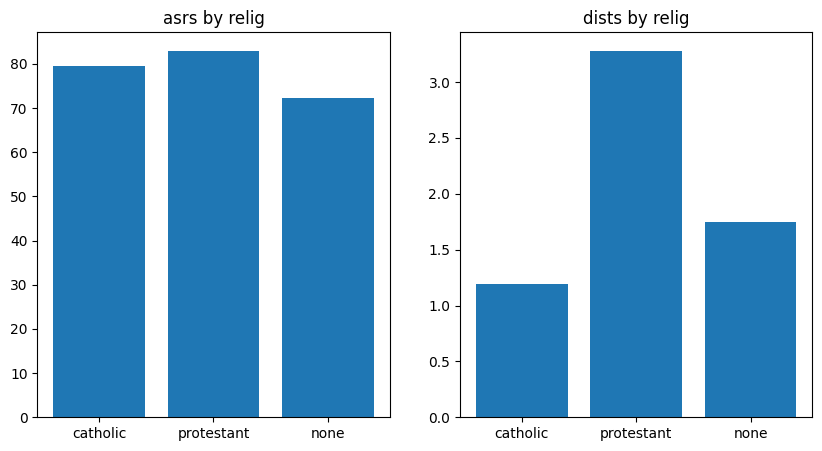
\includegraphics[width=0.33\textwidth]{plots/disparate_vulnerability_3.png}\label{fig:disparate_vulnerability_3}}
    \caption{Disparate vulnerability of the proposed Whitebox attack}
    \label{fig:disparate_vulnerability}
\end{figure}

Figure \ref{fig:disparate_vulnerability} shows the disparate vulnerability of the proposed attack on the GSS dataset.
It also shows the distance between the expected neuron output vector of the positive samples and the negative samples of a subgroup.
The positive sample refers to the sample with the sensitive attribute set to the positive value and the negative sample refers to the sample with the sensitive attribute set to the negative value.
The distance is calculated using the euclidean distance between the expected neuron output vector of the positive samples and the negative samples of a subgroup.
A higher distance indicates the neuron output may be more useful in identifying the sensitive attribute of the subgroup.
The trends in the distance and the disparate vulnerability are similar confirming the above hypothesis.


\section{Focused Attack Results}
\subsection*{Modified Attack Strategy}
\begin{itemize}
    \item Instead of training the attack model on all neuron output features of $M$, the attack model is trained on the subset of features that contribute to $\theta\%$ of the total distance between the positive and negative samples.
\end{itemize}

\subsection*{Results}
% \begin{table}
% \tiny
% \begin{tabular}{p{1cm}p{1cm}p{1cm}p{1cm}p{1cm}p{1cm}p{1cm}p{1cm}p{1cm}p{1cm}}
%     \hline
%     Subgroup Name   & Subgroup Value   &   Original ASR &   Improved Attack ASR (0.5) &   Improved Attack ASR (0.6) &   Improved Attack ASR (0.7) &   Improved Attack ASR (0.8) &   Improved Attack ASR (0.9) &   Improved Attack ASR (0.95) &   Improved Attack ASR (0.99) \\
%     \hline
%      sex             & female           &          63.19 &                       \textbf{67.40} &                       65.46 &                       63.80 &                       64.18 &                       63.70 &                        64.94 &                        65.00 \\
%      sex             & male             &          63.66 &                       \textbf{68.13} &                       66.49 &                       64.93 &                       66.74 &                       65.29 &                        65.10 &                        64.69 \\
%      race            & white            &          64.67 &                       \textbf{68.70} &                       67.04 &                       66.27 &                       66.88 &                       66.09 &                        66.70 &                        67.68 \\
%      race            & other            &          57.62 &                       59.75 &                       \textbf{61.64} &                       59.05 &                       55.40 &                       57.84 &                        60.79 &                        61.28 \\
%      race            & black            &          61.54 &                       59.40 &                       67.87 &                       \textbf{68.68} &                       62.79 &                       61.96 &                        68.08 &                        66.04 \\
%      relig           & catholic         &          61.58 &                       60.89 &                       64.42 &                       63.71 &                       \textbf{66.78} &                       64.68 &                        63.81 &                        62.43 \\
%      relig           & protestant       &          66.95 &                       69.29 &                       69.11 &                       \textbf{69.58} &                       67.49 &                       68.94 &                        68.20 &                        66.50 \\
%      relig           & none             &          61.14 &                       62.27 &                       60.22 &                       61.17 &                       61.41 &                       64.29 &                        \textbf{65.21} &                        60.25 \\
%     \hline
% \end{tabular}
% \caption{ASR of the proposed attack with modified attack strategy}
% \label{tab:asr_improved_attack}
% \end{table}

\begin{table}
    \tiny
    \begin{tabular}{p{1cm}p{1cm}p{1cm}p{1cm}p{1cm}p{1cm}p{1cm}p{1cm}p{1cm}p{1cm}p{1cm}}
        \hline
        Subgroup Name   & Subgroup Value   &   Original ASR &   Improved Attack ASR (0.5) &   Improved Attack ASR (0.6) &   Improved Attack ASR (0.7) &   Improved Attack ASR (0.8) &   Improved Attack ASR (0.9) &   Improved Attack ASR (0.95) &   Improved Attack ASR (0.99) & Correlation Attack ASR \\
        \hline
         sex             & female           &          63.19 &                       \textbf{67.40} &                       65.46 &                       63.80 &                       64.18 &                       63.70 &                        64.94 &                        65.00  & 67.48 \\
         sex             & male             &          63.66 &                       \textbf{68.13} &                       66.49 &                       64.93 &                       66.74 &                       65.29 &                        65.10 &                        64.69 & 64.85 \\
         race            & white            &          64.67 &                       \textbf{68.70} &                       67.04 &                       66.27 &                       66.88 &                       66.09 &                        66.70 &                        67.68 & 68.53 \\
         race            & other            &          57.62 &                       59.75 &                       \textbf{61.64} &                       59.05 &                       55.40 &                       57.84 &                        60.79 &                        61.28 & NA \\
         race            & black            &          61.54 &                       59.40 &                       67.87 &                       \textbf{68.68} &                       62.79 &                       61.96 &                        68.08 &                        66.04 & 78.53 \\
         relig           & catholic         &          61.58 &                       60.89 &                       64.42 &                       63.71 &                       \textbf{66.78} &                       64.68 &                        63.81 &                        62.43 & 66.02 \\
         relig           & protestant       &          66.95 &                       69.29 &                       69.11 &                       \textbf{69.58} &                       67.49 &                       68.94 &                        68.20 &                        66.50 & 71.35 \\
         relig           & none             &          61.14 &                       62.27 &                       60.22 &                       61.17 &                       61.41 &                       64.29 &                        \textbf{65.21} &                        60.25 & 59.23 \\
        \hline
    \end{tabular}
    \caption{ASR of the proposed attack with modified attack strategy}
    \label{tab:asr_improved_attack}
    \end{table}

% {'sex': {'asrs': {'female': 67.48346844995703, 'male': 64.85025207467638}, 'dists': {'female': 0.47285606082663384, 'male': 0.8288567398871771}}, 'race': {'asrs': {'white': 68.5323719683497, 'black': 78.53333333333333}, 'dists': {'white': 0.7485709773756537, 'black': 0.3517112583228034}}, 'relig': {'asrs': {'catholic': 66.02446556965691, 'protestant': 71.35118726389638, 'none': 59.23295454545454}, 'dists': {'catholic': 0.36091806505653895, 'protestant': 0.7454172567814691, 'none': 0.6708013114637875}}}

Table \ref{tab:asr_improved_attack} shows the ASR of the proposed attack with the modified attack strategy with different values of $\theta$.
The ASR of the proposed attack with the modified attack strategy is lower than the ASR of the proposed attack with the original attack strategy.
With higher values of $\theta$, the ASR of the proposed attack with the modified attack strategy is closer to the ASR of the proposed attack with the original attack strategy.

\end{document}